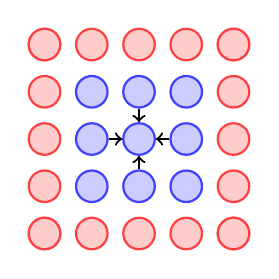
\begin{tikzpicture}[scale=0.6]
\tikzstyle{place}=[circle,thick,draw=blue!75,fill=blue!20,minimum size=4mm]

\node[place] (p1) at (0,0) {};
\node[place] (p2) at (0,1) {};
\node[place] (p3) at (1,0) {};
\node[place] (p4) at (-1,0) {};
\node[place] (p5) at (0,-1) {};

\node[place] () at (-1,-1) {};
\node[place] () at (-1,1) {};
\node[place] () at (1,-1) {};
\node[place] () at (1,1) {};

\draw[->,thick] (p2) to (p1);
\draw[->,thick] (p3) to (p1);
\draw[->,thick] (p4) to (p1);
\draw[->,thick] (p5) to (p1);

\tikzstyle{place}=[circle,thick,draw=red!75,fill=red!20,minimum size=4mm]

\foreach \x in {-2,...,2}
{
  \node[place] () at (\x,2) {};
  \node[place] () at (\x,-2) {};
  \node[place] () at (2,\x) {};
  \node[place] () at (-2,\x) {};
}



\end{tikzpicture}
